\documentclass[professionalfonts, xcolor=table]{beamer}
%% \documentclass[professionalfonts, xcolor=table, handout]{beamer}
%% \usepackage{pgfpages}
%% \pgfpagesuselayout{4 on 1}[a4paper,border shrink=5mm, landscape]
\usepackage{amsmath,amssymb}
\usepackage{txfonts}
\usepackage{fontawesome}
\usepackage{tikz}
\usetikzlibrary{positioning, shapes.multipart, arrows.meta, calc}

\usepackage{fancyvrb}

\usepackage{fontspec}
\defaultfontfeatures{Mapping=tex-text,Scale=MatchLowercase}
\setmainfont{Libertinus Serif}
\setsansfont{Libertinus Sans}
\setmonofont{Menlo Regular}

\usepackage{emoji}

\usetheme{CambridgeUS}

\useinnertheme{circles}
\usecolortheme{orange}
\usefonttheme{serif}

\colorlet{fgcolor}{PUorange!60!black}
\colorlet{bgcolor}{white!85!PUorange}

\setbeamerfont*{frametitle}{series=\bfseries}

\setbeamercolor{alerted text}{fg=red}
\setbeamertemplate{navigation symbols}{}

\setbeamercolor{emphC}{fg=red}
\setbeamercolor{block title}{bg=fgcolor, fg=bgcolor}
\setbeamercolor{block body}{bg=bgcolor, fg=black}
\setbeamercolor{itemize item}{fg=fgcolor}
\setbeamercolor{itemize subitem}{fg=fgcolor}
%% \setbeamercolor{description item}{fg=darkg}

\newcommand{\islock}{\boxdotright}
\newcommand{\treerep}{\ensuremath{\mathsf{bst\_abs}}}
\newcommand{\nodeboxrep}{\ensuremath{\mathsf{bst\_ref}}}
\newcommand{\publichalf}[2]{\ensuremath{\mathsf{node\_ghost}^{.5}_{#1}\left(#2\right)}}
\newcommand{\myhalf}[2]{\ensuremath{\mathsf{node\_ghost}^{.5}_{#1}\left(#2\right)}}
\newcommand{\hide}[1]{}
\newcommand{\emphd}[1]{{\bfseries #1}}
\newcommand{\emphr}[2]{\alert<#1>{#2}}

\title[Proving Logical Atomicity]{Proving Logical Atomicity using Lock Invariants}
\author[Roshan Sharma et al.]{Roshan Sharma \and \underline{Shengyi Wang} \and Alexander Oey \\ Anastasiia Evdokimova \and Lennart Beringer \and William Mansky}
\institute[UIC, Princeton]{
\includegraphics[height=0.08\textwidth]{uic.eps}\hspace{4ex}
\includegraphics[height=0.08\textwidth]{princeton.eps}}
\date{\today}
\begin{document}
\begin{frame}
  \titlepage
\end{frame}

\section{Introduction}
\begin{frame}{What We Have Done}
  \begin{itemize}[<+->]
  \item We use lock invariants to prove logically atomic
    specifications for concurrent data structures.
  \item The proofs are significantly more complicated than those that
    use TaDA-style lock specifications.
  \item This is the first foundational verification of a C
    implementation against logically atomic specifications.
  \end{itemize}
\end{frame}

\section{Background}

\subsection{Two Styles of Lock Specification}

\begin{frame}{Two Styles of Lock Specification}

  \begin{block}{Lock Invariant Style\hfill[Gotsman et al., 2007; Hobor et al., 2008]}
    \vspace*{-\baselineskip}\setlength\belowdisplayshortskip{0pt}
    \begin{gather*}
      \{ \ell \islock R \}\ \texttt{acquire}(\ell)\ \{ R * \ell \islock R \} \\
      \{ R * \ell \islock R \}\ \texttt{release}(\ell)\ \{ \ell \islock R \}
    \end{gather*}
  \end{block}

  \pause

  \begin{block}{TaDA Style\hfill[da Rocha Pinto et al., 2014]}
    \vspace*{-\baselineskip}\setlength\belowdisplayshortskip{0pt}
    \begin{gather*}
      \langle b.\ (\mathsf{L}(\ell) \land \neg b) \vee (\mathsf{U}(\ell) \land b) \rangle\ \texttt{acquire}(\ell)\ \langle \mathsf{L}(\ell) \land b \rangle \\
      \langle \mathsf{L}(\ell) \rangle\ \texttt{release}(\ell)\ \langle \mathsf{U}(\ell) \rangle
    \end{gather*}
  \end{block}

\end{frame}

\subsection{Logically Atomic Specifications}

\begin{frame}{Logically Atomic Specifications}
  \begin{block}{Atomic Triple}
    \centering
    $\langle a.\ P_l\ |\ P_p(a)\rangle\ c\ \langle Q_l\ |\ Q_p(a)\rangle$
  \end{block}

  \pause
  \begin{block}{Example: a specification for \texttt{push}}
    \centering
    \only<2-3>{$\langle s.\ \mathsf{is\_stack}_{\color<3>{red}{g}}\ p\ |\ \mathsf{stack}_{\color<3>{red}{g}}\ s\rangle\ \texttt{push}(v)\ \langle \mathsf{is\_stack}_{\color<3>{red}{g}}\ p\ |\ \mathsf{stack}_{\color<3>{red}{g}}\ (v :: s)\rangle$}
    \only<4>{$\langle s.\ \mathsf{is\_stack}\ p\ |\ \mathsf{stack}\ s\rangle\ \texttt{push}(v)\ \langle \mathsf{is\_stack}\ p\ |\ \mathsf{stack}\ (v :: s)\rangle$}
  \end{block}

\end{frame}

\subsection{VST and Iris}
\begin{frame}{VST and Iris}
  \begin{center}
    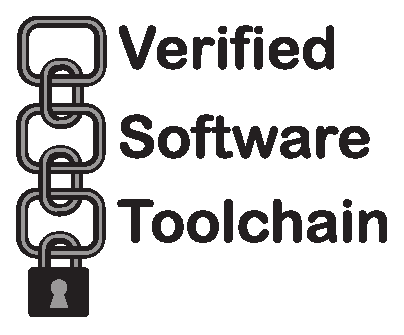
\includegraphics[height=.4\textheight]{vst.eps}
    \hspace{2ex}
    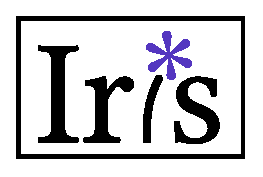
\includegraphics[height=.4\textheight]{iris.eps}
  \end{center}

\end{frame}

\section{Locks and Atomicity}

\begin{frame}[label=bstspec]{Concurrent Binary Search Tree (BST) as an Example}
  \begin{block}{Atomic Specifications}
    \vspace*{-\baselineskip}\setlength\belowdisplayshortskip{0pt}
    \begin{gather*}
      \langle m.\,\nodeboxrep\ p\mid \treerep\ m\rangle\,\texttt{insert}(p, k, v)\,\langle \nodeboxrep\ p\mid \treerep\ (m[k \mapsto v])\rangle\\
      \langle m.\,\nodeboxrep\ p\mid \treerep\ m\rangle\,\texttt{lookup}(p, k)\,\langle v.\,\nodeboxrep\ p\mid \treerep\ m \land m(k) = v\rangle\\
      \langle m.\,\nodeboxrep\ p\mid \treerep\ m\rangle\,\texttt{delete}(p, k)\,\langle \nodeboxrep\ p\mid \treerep\ (m[k \mapsto \_])\rangle
    \end{gather*}
  \end{block}
\end{frame}

\subsection{Coarse-Grained Locking}
\begin{frame}{Coarse-Grained Locking}
  \begin{block}{Definitions of Data Structure Assertions}
    \vspace*{-\baselineskip}\setlength\belowdisplayshortskip{0pt}
    \begin{align*}
      R_{\mathit{cg}} &\triangleq \exists t.\ \mathsf{BST}\ p\ t * \mathsf{ghost\_bst}_{.5}\ t\\
      \nodeboxrep\ l &\triangleq l \islock_\pi R_{\mathit{cg}}\\
      \treerep\ t &\triangleq \mathsf{ghost\_bst}_{.5}\ t
    \end{align*}
  \end{block}
\end{frame}

\begin{frame}{Sketch Proof of Coarse-Grained Insertion of BST}
  \centering
  \begin{tikzpicture}[node distance=0.3mm]
    \node (line 0) {\color<3->{lightgray}{$\langle l \islock_\pi R_{\mathit{cg}} \mid \mathsf{ghost\_bst}_{.5}t \rangle$}};
    \onslide<2->{\node (line 1) [below = of line 0]
      {\color<4->{lightgray}{$\langle l \islock_\pi (\exists t.\ \mathsf{BST}\ p\ t * \mathsf{ghost\_bst}_{.5}\ t) \mid \mathsf{ghost\_bst}_{.5}t \rangle$}};}
    \node (line 2) [below = of line 1] {\color<2,4->{lightgray}{\Verb|acquire(l);|}};
    \onslide<3->{\node (line 3) [below = of line 2]
      {\color<5->{lightgray}{$\langle \mathsf{BST}\ p\ t_1 * \mathsf{ghost\_bst}_{.5}t_1 * l \islock_\pi R_{\mathit{cg}} \mid \mathsf{ghost\_bst}_{.5}t \rangle$}};}
    \onslide<4->{\node (line 4) [below = of line 3] {\color<6->{lightgray}{$\{ \mathsf{BST}\ p\ t_1 \}$}};}
    \node (line 5) [below = of line 4] {\color<2-4,6->{lightgray}{\Verb|seq\_insert(p, x, v);|}};
    \onslide<5->{\node (line 6) [below = of line 5] {\color<7->{lightgray}{$\{ \mathsf{BST}\ p\ t_1[x\mapsto v]\}$}};}
    \onslide<6->{\node (line 7) [below = of line 6] {\color<8->{lightgray}{$\langle \mathsf{BST}\ p\ t_1[x\mapsto v] * \mathsf{ghost\_bst}_{.5}t_1 * l \islock_\pi R_{\mathit{cg}} \mid \mathsf{ghost\_bst}_{.5}t \rangle$}};}
    \onslide<7->{\node (line 8) [below = of line 7]
      {$\langle \mathsf{BST}\ p\ t[x\mapsto v] * \mathsf{ghost\_bst}_{.5}t[x\mapsto v] * l \islock_\pi R_{\mathit{cg}} \mid \mathsf{ghost\_bst}_{.5}\ t[x\mapsto v]\rangle$};}
    \node (line 9) [below = of line 8] {\color<2-7>{lightgray}{\Verb|release(l);|}};
    \onslide<1-8>{\node (line 10) [below = of line 9] {\color<2-7>{lightgray}{$\langle l \islock_\pi R_{\mathit{cg}} \mid \mathsf{ghost\_bst}_{.5}\ t[x\mapsto v]\rangle$}};}
  \end{tikzpicture}
\end{frame}

\subsection{Hand-over-Hand Locking}

\begin{frame}{Fine-Grained Locking: General Idea}
  \begin{itemize}[<+->]
  \item There are multiple locks on different pieces of the data structure
  \item A ghost state represents the abstract state of a locked section alone
  \item The abstract state of the data structure is derived from the composition of the states of the locked components
  \item Each locked component $c$ has a piece of ghost state
    $\mathsf{ghost}\_c$ that is split between the lock invariant and
    the top-level abstract state
  \item The lock invariant for each component must also carefully
    account for the ownership of both that component’s lock and the
    locks of related nodes
  \end{itemize}
\end{frame}

\hide{

\begin{frame}{Hand-over-Hand Locking: Linked-List Example}
  \pause
  \begin{block}{Normal Lock Invariant}
    \centering
    $R(n) \triangleq n \mapsto (d, n', \ell') * \ell' \islock_\pi R(n')$
  \end{block}
  \pause
  \begin{block}{}
    \vspace*{-\baselineskip}\setlength\belowdisplayshortskip{0pt}
    \begin{gather*}
      \{ \ell \islock R \}\ \texttt{acquire}(\ell)\ \{ R * \ell \islock R \} \\
      \{ R * \ell \islock R \}\ \texttt{release}(\ell)\ \{ \ell \islock R \}
    \end{gather*}
  \end{block}
  \pause
  \begin{block}{}
    \vspace*{-\baselineskip}\setlength\belowdisplayshortskip{0pt}
    \begin{gather*}
      \{ \ell \islock_\pi R(n) * n \mapsto (d, n', \ell') * \ell' \islock_\pi R(n') \}\\
      \texttt{acquire}(\ell');\\
      \{ \ell \islock_\pi R(n) * n \mapsto (d, n', \ell') * \ell' \islock_\pi R(n') * \null \\\ n' \mapsto (d, n'', \ell'') * \ell'' \islock_\pi R(n'') \}\\
      \texttt{release}(\ell);\\
      \{ \ell \islock_\pi R(n) * n' \mapsto (d, n'', \ell'') * \ell'' \islock_\pi R(n'') \}
    \end{gather*}
  \end{block}
\end{frame}

\begin{frame}{Hand-over-Hand Locking: Linked-List Example}
  \begin{block}{Recursive Lock Invariant}
    \centering
    $R(n) \triangleq \ell \islock_{\pi_1} R(n) * n \mapsto (d, n', \ell') * \ell' \islock_{\pi_2} R(n')$
  \end{block}
  \pause
  \begin{block}{}
    \vspace*{-\baselineskip}\setlength\belowdisplayshortskip{0pt}
    \begin{gather*}
      \{ \ell \islock R \}\ \texttt{acquire}(\ell)\ \{ R * \ell \islock R \} \\
      \{ R * \ell \islock R \}\ \texttt{release}(\ell)\ \{ \ell \islock R \}
    \end{gather*}
  \end{block}
  \begin{block}{}
    \vspace*{-\baselineskip}\setlength\belowdisplayshortskip{0pt}
    \begin{gather*}
      \{ \ell \islock_{\pi_1} R(n) * n \mapsto (d, n', \ell') * \ell' \islock_{\pi_2} R(n') \}\\
      \texttt{acquire}(\ell');\\
      \{ \ell \islock_{\pi_1} R(n) * n \mapsto (d, n', \ell') * \ell' \islock_{\pi_2} R(n')\ * \\
      \ \ell' \islock_{\pi_1} R(n') * n' \mapsto (d, n'', \ell'') * \ell'' \islock_{\pi_2} R(n'') \}\\
      \texttt{release}(\ell);\\
      \{ \ell' \islock_{\pi_1} R(n') * n' \mapsto (d, n'', \ell'') * \ell'' \islock_{\pi_2} R(n'') \}
    \end{gather*}
  \end{block}
\end{frame}

}

\tikzset{
    onslide/.code args={<#1>#2}{\only<#1>{\pgfkeysalso{#2}}}
  }

\begin{frame}[fragile]{Hand-over-Hand Locking: BST Example}
  \begin{columns}[c]
    \column{.3\textwidth}
  \centering
  \begin{tikzpicture}[thick, nd/.style={thick, circle, draw, text=black}]
    \node [onslide=<1>{PUorange}, onslide=<4->{PUorange}, onslide=<2-3>{blue}, nd] (n30) {30}
    child [onslide=<1>{PUorange}, onslide=<4->{PUorange}, onslide=<2-3>{blue}] {node [PUorange, nd] (n25) {25}}
    child [onslide=<1>{PUorange}, onslide=<4->{PUorange}, onslide=<2-3>{blue}] {node [onslide=<1-2>{PUorange}, onslide=<3-5>{blue}, nd] (n75) {75}
      child [onslide=<1-2>{PUorange}, onslide=<6>{PUorange}, onslide=<3-5>{blue}] { node [onslide=<1-4>{PUorange}, onslide=<5-7>{blue}, nd] (n40) {40}
        child [onslide=<1-4>{PUorange}, onslide=<8->{PUorange}, onslide=<5-7>{blue}] {node [onslide=<1-6>{PUorange}, onslide=<7-8>{blue}, nd] (n35) {35}}
        child [onslide=<1-4>{PUorange}, onslide=<8->{PUorange}, onslide=<5-7>{blue}] {node [PUorange, nd] (n55) {55}
          child [PUorange] {node [nd] (n50) {50}}
          child [PUorange] {node [nd] (n60) {60}}}}
      child [onslide=<1-2>{PUorange}, onslide=<3-5>{blue}] { node [PUorange, nd] (n80) {80} }
    };
    \onslide<1,4->{\node [PUorange] at (n30.north west) {\faLock};}
    \onslide<2-3>{\node [blue] at (n30.north west) {\faUnlock};}
    \node [PUorange] at (n25.north west) {\faLock};
    \onslide<1-2,6->{\node [PUorange] at (n75.north west) {\faLock};}
    \onslide<3-5>{\node [blue] at (n75.north west) {\faUnlock};}
    \onslide<1-4, 8->{\node [PUorange] at (n40.north west) {\faLock};}
    \onslide<5-7>{\node [blue] at (n40.north west) {\faUnlock};}
    \node [PUorange] at (n80.north west) {\faLock};
    \onslide<1-6,9>{\node [PUorange] at (n35.north west) {\faLock};}
    \onslide<7-8>{\node [blue] at (n35.north west) {\faUnlock};}
    \node [PUorange] at (n55.north west) {\faLock};
    \node [PUorange] at (n50.north west) {\faLock};
    \node [PUorange] at (n60.north west) {\faLock};
  \end{tikzpicture}
  \column{.7\textwidth}
  \centering
  \begin{tikzpicture}
    \node [rectangle, fill=bgcolor] {
\begin{BVerbatim}[commandchars=\\\[\]]
\emphd[void] *lookup (\emphd[treebox] t, \emphd[int] x) {
  \emphr[2][acquire(l);] p = tgt->t;
  \emphd[while] (p != NULL) {
    \emphd[int] y = p->key;
    \emphd[if] (x < y) {
      tgt = p->left; \emphd[void] *l_old = l;
      l = tgt->lock; \emphr[5,7][acquire(l);]
      p=tgt->t; \emphr[6,8][release(l_old);]
    } \emphd[else if] (y < x) {
      tgt=p->right; \emphd[void] *l_old = l;
      l = tgt->lock; \emphr[3][acquire(l);]
      p=tgt->t; \emphr[4][release(l_old);]
    } \emphd[else] {
      v = p->value; \emphr[9][release(l); \emphd[return] v;]
    } ... }
\end{BVerbatim}
  };
  \end{tikzpicture}
  \end{columns}
\end{frame}

\hide {
  \begin{tikzpicture}
    \filldraw [fill=bgcolor, draw=black] (0,0) rectangle (5, 7);
    \onslide<1>{\node at (2.5, 3.5) {$\mathsf{node\_inv}_g(p)$};}
    \onslide<2>{
      \node at (1.25, 1.75) {$\mathsf{node\_inv}_{g_l}$};
      \node at (3.75, 1.75) {$\mathsf{node\_inv}_{g_r}$};}
    \onslide<2->{
      \draw (0, 3.5) -- (5, 3.5);
      \draw (2.5, 0) -- (2.5, 3.5);
      \node at (2.5, 5.25) {
        $\begin{gathered}
          \exists i\ j\ c.\ \mathsf{node\_ghost}_{g}^{.5}\left(c, (i, j)\right) * \null\\
          p.\mathsf{lock} \islock_{\pi_1}\mathsf{node\_inv}_g
        \end{gathered}$
      };
    }
    \onslide<3->{
      \draw (0, 1.75) -- (5, 1.75);
      \draw (1.25, 0) -- (1.25, 1.75);
      \draw (3.75, 0) -- (3.75, 1.75);
      \node at (1.25, 2.625) {\scriptsize
        $\begin{gathered}
          \exists \dots * \null\\
          p_l\islock_{\pi_1}\mathsf{node\_inv}_{g_l}
        \end{gathered}$};
      \node at (3.75, 2.625) {\scriptsize
        $\begin{gathered}
          \exists \dots * \null\\
          p_r\islock_{\pi_1}\mathsf{node\_inv}_{g_r}
        \end{gathered}$};
    }
    \onslide<3>{
      \node at (0.625, 0.875) {\tiny $\mathsf{node\_inv}_{g_{ll}}$};
      \node at (1.875, 0.875) {\tiny $\mathsf{node\_inv}_{g_{lr}}$};
      \node at (3.125, 0.875) {\tiny $\mathsf{node\_inv}_{g_{rl}}$};
      \node at (4.375, 0.875) {\tiny $\mathsf{node\_inv}_{g_{rr}}$};
    }
    \onslide<4->{
      \draw (0, 0.875) -- (5, 0.875);
      \draw (0.625, 0) -- (0.625, 0.875);
      \draw (1.875, 0) -- (1.875, 0.875);
      \draw (3.125, 0) -- (3.125, 0.875);
      \draw (4.375, 0) -- (4.375, 0.875);
      \node at (0.625, 1.3125) {\tiny $\begin{gathered}\exists \dots * \null\\ \mathsf{node\_inv}_{g_{ll}}\end{gathered}$};
      \node at (1.875, 1.3125) {\tiny $\begin{gathered}\exists \dots * \null\\ \mathsf{node\_inv}_{g_{lr}}\end{gathered}$};
      \node at (3.125, 1.3125) {\tiny $\begin{gathered}\exists \dots * \null\\ \mathsf{node\_inv}_{g_{rl}}\end{gathered}$};
      \node at (4.375, 1.3125) {\tiny $\begin{gathered}\exists \dots * \null\\ \mathsf{node\_inv}_{g_{rr}}\end{gathered}$};
      \node at (0.3125, 0.4375) {\tiny $\cdots$};
      \node at (0.9375, 0.4375) {\tiny $\cdots$};
      \node at (1.5625, 0.4375) {\tiny $\cdots$};
      \node at (2.1875, 0.4375) {\tiny $\cdots$};
      \node at (2.8125, 0.4375) {\tiny $\cdots$};
      \node at (3.4375, 0.4375) {\tiny $\cdots$};
      \node at (4.0625, 0.4375) {\tiny $\cdots$};
      \node at (4.6875, 0.4375) {\tiny $\cdots$};
    }
  \end{tikzpicture}
}

\begin{frame}{Recursive Lock Invariant}
  \begin{columns}[c]
    \column{.3\textwidth}
    \centering
    \begin{tikzpicture}[thick, nd/.style={thick, circle, draw, text=black},
        ->/.style={-Stealth}]
      \node [PUorange, nd] (n30) {30}
      child [PUorange] {node [nd] (n25) {25}}
      child [PUorange] {node [nd] (n75) {75}
        child { node [nd] (n40) {40}
          child { node [nd] (n35) {35}}
          child {node [nd] (n55) {55}
            child {node [nd] (n50) {50}}
            child {node [nd] (n60) {60}}}}
        child { node [nd] (n80) {80} }
      };
      \node [PUorange] at (n30.north west) {\faLock};
      \node [PUorange] at (n25.north west) {\faLock};
      \node [PUorange] at (n75.north west) {\faLock};
      \node [PUorange] at (n40.north west) {\faLock};
      \node [PUorange] at (n80.north west) {\faLock};
      \node [PUorange] at (n35.north west) {\faLock};
      \node [PUorange] at (n55.north west) {\faLock};
      \node [PUorange] at (n50.north west) {\faLock};
      \node [PUorange] at (n60.north west) {\faLock};

      \onslide<2->{
        \node [PUorange, inner sep=0pt] at (n30.north east) (l30) {\faSquare};
        \node [PUorange, inner sep=0pt] at (n25.north east) (l25) {\faSquare};
        \node [PUorange, inner sep=0pt] at (n75.north east) (l75) {\faSquare};
        \node [PUorange, inner sep=0pt] at (n40.north east) (l40) {\faSquare};
        \node [PUorange, inner sep=0pt] at (n80.north east) (l80) {\faSquare};
        \node [PUorange, inner sep=0pt] at (n35.north east) (l35) {\faSquare};
        \node [PUorange, inner sep=0pt] at (n55.north east) (l55) {\faSquare};
        \node [PUorange, inner sep=0pt] at (n50.north east) (l50) {\faSquare};
        \node [PUorange, inner sep=0pt] at (n60.north east) (l60) {\faSquare};
      }

      \onslide<3->{
        \draw [->, blue] (l30.south) ..controls +(0, -0.6)..(l25);
        \draw [->, blue] (l30) -- (l75);
        \draw [->, blue] (l75.south) ..controls +(0, -0.6)..(l40);
        \draw [->, blue] (l75) -- (l80);
        \draw [->, blue] (l40.south) ..controls +(0, -0.6)..(l35);
        \draw [->, blue] (l40) -- (l55);
        \draw [->, blue] (l55.south) ..controls +(0, -0.6)..(l50);
        \draw [->, blue] (l55) -- (l60);
        \draw [->, blue] (l30.east) ..controls +(0.5,0.2) and +(0.2,0.5)..(l30.north);
        \draw [->, blue] (l75.east) ..controls +(0.5,0.2) and +(0.2,0.5)..(l75.north);
        \draw [->, blue] (l40.east) ..controls +(0.5,0.2) and +(0.2,0.5)..(l40.north);
        \draw [->, blue] (l55.east) ..controls +(0.5,0.2) and +(0.2,0.5)..(l55.north);
      }
  \end{tikzpicture}
    \column{.65\textwidth}
    \centering
    \begin{block}<4->{Lock Invariant: $\text{\color{PUorange}\faSquare}_g(p)$}
      \vspace*{-\baselineskip}\setlength\belowdisplayshortskip{0pt}
      \begin{align*}
        \text{\color{PUorange}\faSquare}_g(p) \triangleq \ &\exists i\,j\ c.\ \text{\emoji{ghost}}_g^{.5}\left((i, j), c\right) * \null\\
        & p.\texttt{lock}\ {\color{blue}\islock_{\pi_1}} \text{\color{PUorange}\faSquare}_g * \null\\
        &\mathsf{match}\ c\ \mathsf{with}\\
        &|\ \mathsf{None} \Rightarrow p.\texttt{t} = \texttt{NULL}\\
        &|\ \mathsf{Some}\ (k, v, g_l, g_r) \Rightarrow k \in (i, j) \land \null\\
        &\qquad \exists p_l, p_r.\ p.\texttt{t} \mapsto (k, v, p_l, p_r) * \null \\
        &\qquad p_l.\texttt{lock}\ {\color{blue}\islock_{\pi_2}} \text{\color{PUorange}\faSquare}_{g_l} * \null\\
        &\qquad p_r.\texttt{lock}\ {\color{blue}\islock_{\pi_2}} \text{\color{PUorange}\faSquare}_{g_r}
      \end{align*}
    \end{block}
    \begin{block}<5->{Per-Thread Handle to the BST}
      \centering
      $\nodeboxrep_g\,b \triangleq \exists p.\ b \mapsto p * p.\texttt{lock} \islock \text{\color{PUorange}\faSquare}_g(p)$
    \end{block}
  \end{columns}
\end{frame}

\begin{frame}<1-3>[label=ghost]{Global Ghost State: $\treerep_g$}
  \begin{columns}[c]
    \column{.54\textwidth}
    \centering
    \begin{tikzpicture}[
        level distance=8ex,
        sibling distance=15ex,
        thick,
        nd/.style={thick, rounded corners, PUorange, draw, text=black, rectangle split, rectangle split horizontal, rectangle split parts=2},
        edge from parent/.style={draw, PUorange}]
      \node [nd] (n30) {30\nodepart{two}\color{fgcolor}$(-\infty, \infty)$}
      child {node [nd] (n25) {25\nodepart{two}\color{fgcolor}$(-\infty, 30)$}}
      child { node [nd] (n75) {75\nodepart{two}\color{fgcolor}$(30, \infty)$}
        child { node [nd] (n40) {40\nodepart{two}\color{fgcolor}$(30, 75)$}
          child { node [nd] (n35) {35\nodepart{two}\color{fgcolor}$(30, 40)$}}
          child  {node [nd] (n55) {55\nodepart{two}\color{fgcolor}$(40, 75)$}
            child {node [nd] (n50) {50\nodepart{two}\color{fgcolor}$(40, 55)$}}
            child {node [nd] (n60) {60\nodepart{two}\color{fgcolor}$(55,75)$}}}}
        child  { node [nd] (n80) {80\nodepart{two}\color{fgcolor}$(75,\infty)$} }
      };
    \end{tikzpicture}
    \column{.43\textwidth}
    \begin{block}<2->{}
      \vspace*{-\baselineskip}\setlength\belowdisplayshortskip{0pt}
      \begin{align*}
        & \text{\color{PUorange}\faSquareO}_g\left(t, (i, j)\right) \triangleq\\
        & \;\mathsf{match}\ t\ \mathsf{with}\\
        & \;|\ \mathsf{Leaf} \Rightarrow \text{\emoji{ghost}}_g^{.5}\left((i, j), \mathsf{None}\right)\\
        & \;|\ \mathsf{Node}\ (k, v, t_l, g_l, t_r, g_r) \Rightarrow\\
        & \;\; \text{\emoji{ghost}}_g^{.5}\left((i, j), \mathsf{Some}\ (k, v, g_l, g_r)\right) * \null \\
        & \;\; \text{\color{PUorange}\faSquareO}_{g_l}\left(t_l, (i, k)\right) * \text{\color{PUorange}\faSquareO}_{g_r}\left(t_r, (k, j)\right)
      \end{align*}
    \end{block}
    \begin{block}<3->{}
      \vspace*{-\baselineskip}\setlength\belowdisplayshortskip{0pt}
      \begin{align*}
        & \treerep_g\ m \triangleq\ \exists t.\ {\color<4>{red}{t \textrm{ impl } m}} \land \null\\
        & \text{\color{PUorange}\faSquareO}_g\left(t, (-\infty, +\infty)\right) * \null \\
        &\mathsf{ghost\_nodes}\left(\mathrm{ids}(t)\right)
      \end{align*}
    \end{block}
  \end{columns}
\end{frame}

\begin{frame}{BST Rotation}
  \centering
  \begin{tikzpicture}
    [thick, sibling distance=12ex,
      nd/.style={thick, circle, draw, text=black}]
    \only<1-2>{
      \node [PUorange, nd] (n30) {30}
      child [PUorange] {node [nd] (n25) {25}}
      child [PUorange] {node [nd] (n75) {75}
        child { node [nd, onslide=<2->{blue}] (n40) {40}
          child { node [nd] (n35) {35}
            child [transparent] {node [nd] (nt1) {35}}
            child [transparent] {node [nd] (nt2) {35}}}
          child {node [nd, onslide=<2>{blue}] (n55) {55}
            child {node [nd] (n50) {50}}
            child {node [nd] (n60) {60}}}}
        child { node [nd] (n80) {80} }
      };
    }
    \only<2>{
      \draw[ultra thick, blue, -{>[width=8pt]}] ($ (n35)!.5!(n55) + (0, 2ex) $) +(-75:2.5ex) arc(-75:255:2.5ex);
    }
    \only<3->{
      \node [PUorange, nd] (r30) {30}
      child [PUorange] {node [nd] (r25) {25}}
      child [PUorange] {node [nd] (r75) {75}
        child { node [nd, blue] (r55) {55}
          child {node [nd, blue] (r40) {40}
            child {node [nd] (r35) {35}}
            child {node [nd] (r50) {50}}}
          child { node [nd] (r60) {60}}}
        child { node [nd] (r80) {80} }
      }; }
  \end{tikzpicture}
\end{frame}

\againframe<4>{ghost}

\againframe<2>{bstspec}

\begin{frame}{Comparison with TaDA-Style Specifications}
  \begin{itemize}[<+->]
  \item The key elements of the proof are:
    \begin{itemize}[<+->]
    \item Per-node ghost state for each lock invariant, and global ghost state that summarizes all the per-node state
    \item Complex share accounting for hand-over-hand locking: each
      lock invariant needs to contain a share of itself and shares of
      its child locks
    \end{itemize}
  \item Compare to the template proofs for hand-over-hand locking, which use TaDA-style lock specs:
    \begin{itemize}[<+->]
    \item Still need per-node ghost state and connection to global ghost state
    \item No share accounting: locks are part of the global ghost state and are accessed atomically, never owned by any thread
    %% \item Side note: also, lock can be allocated in one place and given an invariant later (useful in template style)
    \end{itemize}
  \end{itemize}
\end{frame}

\section{Conclusion}
\begin{frame}{Conclusion}
  \begin{itemize}[<+->]
  \item Invariant-based specs can still be used to prove logically
    atomic specs for \emph{fine-grained} locking, with the same
    approach to ghost state as has been used in the TaDA style.
  \item It is more complex than using TaDA-style atomic lock specs: per-node ghost state, complex share accounting
  \item There might be systems where the old lock specs are necessary
    (e.g. in VST they were part of the soundness proof), so it’s good
    to know that we can still prove atomic specs for data structures.
  \item We have just modified VST to support TaDA-style lock specs
    instead, and are looking forward to simpler atomicity proofs for
    fine-grained C programs.
  \end{itemize}
\end{frame}

\end{document}
